% ******************************************************** %
%              TEMPLATE DE INFORME ORGA2 v0.1              %
% ******************************************************** %
% ******************************************************** %
%                                                          %
% ALGUNOS PAQUETES REQUERIDOS (EN UBUNTU):                 %
% ========================================
%                                                          %
% texlive-latex-base                                       %
% texlive-latex-recommended                                %
% texlive-fonts-recommended                                %
% texlive-latex-extra?                                     %
% texlive-lang-spanish (en ubuntu 13.10)                   %
% ******************************************************** %


\documentclass[a4paper]{article}
\usepackage[spanish]{babel}
\usepackage[utf8]{inputenc}
\usepackage{charter}   % tipografia
\usepackage{graphicx}
%\usepackage{makeidx}
\usepackage{paralist} %itemize inline

%\usepackage{float}
%\usepackage{amsmath, amsthm, amssymb}
%\usepackage{amsfonts}
%\usepackage{sectsty}
%\usepackage{charter}
%\usepackage{wrapfig}
%\usepackage{listings}
%\lstset{language=C}

% \setcounter{secnumdepth}{2}
\usepackage{underscore}
\usepackage{caratula}
\usepackage{url}


% ********************************************************* %
% ~~~~~~~~              Code snippets             ~~~~~~~~~ %
% ********************************************************* %

\usepackage{color} % para snipets de codigo coloreados
\usepackage{fancybox}  % para el sbox de los snipets de codigo

\definecolor{litegrey}{gray}{0.94}

\newenvironment{codesnippet}{%
	\begin{Sbox}\begin{minipage}{\textwidth}\sffamily\small}%
	{\end{minipage}\end{Sbox}%
		\begin{center}%
		\vspace{-0.4cm}\colorbox{litegrey}{\TheSbox}\end{center}\vspace{0.3cm}}



% ********************************************************* %
% ~~~~~~~~         Formato de las páginas         ~~~~~~~~~ %
% ********************************************************* %

\usepackage{fancyhdr}
\pagestyle{fancy}

%\renewcommand{\chaptermark}[1]{\markboth{#1}{}}
\renewcommand{\sectionmark}[1]{\markright{\thesection\ - #1}}
%\renewcommand{\sectionmark}[1]{\markright{#1}}

\fancyhf{}

\fancyhead[LO]{Sección \rightmark} % \thesection\ 
\fancyfoot[LO]{\small{Leandro Ezequiel Vigali}}
\fancyfoot[RO]{\thepage}
\renewcommand{\headrulewidth}{0.5pt}
\renewcommand{\footrulewidth}{0.5pt}
\setlength{\hoffset}{-0.8in}
\setlength{\textwidth}{16cm}
%\setlength{\hoffset}{-1.1cm}
%\setlength{\textwidth}{16cm}
\setlength{\headsep}{0.5cm}
\setlength{\textheight}{25cm}
\setlength{\voffset}{-0.7in}
\setlength{\headwidth}{\textwidth}
\setlength{\headheight}{13.1pt}

\renewcommand{\baselinestretch}{1.1}  % line spacing

% ******************************************************** %


\begin{document}


\thispagestyle{empty}
\materia{Organización del Computador II}
\submateria{Segundo Cuatrimestre de 2020}
\titulo{Trabajo Práctico II}
\hspace{20cm}
\subtitulo{Procesamiento SIMD}
\integrante{Leandro Ezequiel Vigali}{951/12}{levleandro@gmail.com}


\maketitle
\newpage

%\thispagestyle{empty}
%\vfill
%\begin{abstract}
%En el presente trabajo se describe la problemática de ...
%\end{abstract}

\thispagestyle{empty}
\vspace{3cm}
\tableofcontents
\newpage


%\normalsize
\newpage

\section{Introducción}

El objetivo de este trabajo práctico consiste en poner en práctica el modelo de procesamiento \textbf{SIMD} (Single Instruction, Multiple Data), que nos ofrece la microarquitectura \textbf{INTEL64}. Este modelo nos permite programar en forma paralela a nivel de datos, es decir, realizar una misma operación sobre un conjunto de datos. A diferencia del modelo \textbf{SISD} (Single Instruction, Single Data) que opera de forma escalar, es decir, un dato por instrucción. \\
Cada una de estas instrucciones interpreta los datos en un tamaño particular, sin importar lo que estos representen. 

\begin{figure}[h]
  \begin{center}
	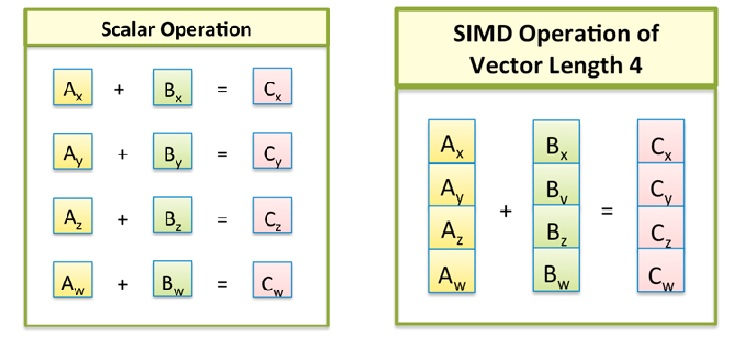
\includegraphics[scale=0.66]{img/simd.jpg}
	\caption{Representación modelo SISD y SIMD}
	\label{simd}
  \end{center}
\end{figure}

\bigskip

La forma en la que se pone en práctica este modelo es mediante la programación y aplicación de filtros sobre imágenes codificados en lenguaje ensamblador.
Las imágenes utilizadas estarán en formato BMP y trandrán un ancho múltiplo de 8 y mayor a 16.
Cada implementación tendrá como objetivo procesar las imágenes de a dos o más pixeles por ciclo.
La Cátedra provee los algoritmos y código C de cada filtro, junto al framework para leer y escribir las imágenes, compilar y testear los resultados obtenidos. Por lo que programarlos en assembler es la primer parte del trabajo.

\bigskip

La otra parte del trabajo consiste en realizar un análisis experimental del funcionamiento de los filtros para entender y razonar sobre el modelo \textbf{SIMD}. Con ese objetivo se realizaron dos experimentos, que fueron desarrollados y analizados, llegando a una conclusión respecto a los resultados obtenidos y los esperados.


\bigskip

{\centering\textbf{\large{Sobre el formato BMP}}} 

\medskip

El formato BMP tiene un encabezado y un mapa de bits que representa la información de los pixeles. La biblioteca provista soporta tres tipos de formatos, con o sin transparencia, estos formatos corresponden a los tipos de encabezados BITMAPINFOHEADER (40 bytes), BITMAPV3INFOHEADER (56 bytes) y BITMAPV5HEADER (124 bytes).
En este tipo de imágenes, el mapa de bits está almacenado de forma que las líneas de la imagen están invertidas, es decir la primera fila de la imagen, se encuentra la última línea. En cada línea los pixeles se almacenan de izquierda a derecha. Pero el framework provisto invierte las líneas para operar con la imagen de forma ordenada.Gracias a dicho framework, podremos tratar cada pixel como un elemento de la imagen vista como una matriz.
Cada pixel posee 4 componentes de tamaño 1 byte cada uno en el siguiente orden: azul (b), verde (g), rojo (r) y transparencia (a).
Las funciones implementadas reciben un puntero al primer pixel correspondiente a la posición [0,0] de la imagen fuente, así también para la imagen destino que contendrá los valores  correspondientes de aplicar el filtro a los pixeles fuentes.
En todos los casos el valor de la transparencia (a) será 255.

\section{Desarrrollo}

\subsection{Parámetros de las funciones}
La siguiente serie de parámetros son provistos a todos los filtros en el siguiente orden:
\begin{itemize}
    \item \textbf{- src:} puntero al inicio de la matriz de pixeles de la imagen entrada
    \item \textbf{- dst:} puntero al inicio de la matriz de pixeles de la imagen salida
    \item \textbf{- height:} representa el alto (cantidad de filas) en pixeles de la imagen, tanto de entrada como de salida
    \item \textbf{- width:} representa el ancho (cantidad de columnas) en pixeles de la imagen, tanto entrada como salida
    \item \textbf{- src_row_size y dst_row_size:} representa el ancho en bytes de cada fila.
\end{itemize}
 Cualquier otro parámetro adicional será particular de cada filtro.


\subsection{Imagen Fantasma}
Este filtro consiste en generar una imagen fantasma utilizando parte de la imagen original en escala de grises y al doble de su tamaño. La parte utilizada será de tamaño ancho/2 x alto/2, y se pasará por parámetro un offset en x e y, que determinará cuál será la imagen fantasma. Cabe aclarar que el rango de los offsets están entre 0 y ancho/2 +1. Si no se pasa ningún offset, el predeterminado es 0, si se pasa algún valor fuera de rango se utilizará el máximo o mínimo offset según corresponda.

\subsubsection{Pseudocódigo del ciclo:}
\begin{codesnippet}
\begin{verbatim}
Para i de 0 a height - 1;
    Para j de 0 a width - 1; 
        int ii = i/2 + offsetY;
        int jj = i/2 + offsetX;
        float b = (src_matrix[ii][jj].r + 2 * src_matrix[ii][jj].g + src_matrix[ii][jj].b) / 4;
        dst_matrix[i][j].r = SATURAR(src_matrix[i][j].r * 0.9 + b/2);
        dst_matrix[i][j].g = SATURAR(src_matrix[i][j].g * 0.9 + b/2);
        dst_matrix[i][j].b = SATURAR(src_matrix[i][j].b * 0.9 + b/2);
\end{verbatim}
\end{codesnippet}

\subsubsection{Implementación del ciclo en ASM}
Como este filtro opera con todos los pixeles, se recorren desde el primer al último pixel de las imágenes de a dos pixeles por ciclo. Paralelamente voy recorriendo la submatriz fantasma de a un pixel por ciclo, con la ayuda de un registro que contendrá la dirección de memoria correspondiente al \textbf{offsetX} e \textbf{offsetY}. 
Pero a diferencia de la matriz fuente y destino, en la submatriz fantasma las filas se recorren dos veces consecutivamente. \\
Adicionalmente se declaran en memoria los siguientes datos floats que para realizar los cálculos necesarios: 
\begin{codesnippet}
\begin{verbatim}   
    mul09:  dd 0.9, 0.9, 0.9, 1.0 
    calc_b: dd 1.0, 2.0, 1.0, 0.0 
    div8:   dd 8.0, 8.0, 8.0, 8.0 
\end{verbatim}
\end{codesnippet}

{\centering\textbf{Cálculo de b/2:}}

Se carga en un registro \textbf{XMM} el pixel apuntado de la submatriz fantasma, es decir leo 4 bytes. \\
Se desempaqueta dos veces la parte baja del registro, es decir el pixel pasó de tener 4 componentes de 1 byte, a 4 componentes de 2 bytes y luego pasasaron a ser de 4 bytes, para convertirlos al tipo float. \\
El siguiente paso es multiplicar el registro por la máscara [calc\_b] para dejar la transparencia en 0 momentáneamente y tener el doble valor de la componente G. \\
Luego se realizan dos sumas horizontales, sobre el mismo registro, obteniendo 4 floats con el mismo valor como se puede ver en la figura~\ref{sumah}. \\
Luego se shiftea 4 bytes a la derecha para dejar en 0's el último float, que se corresponde con tener la transparencia en 0.
Finalmente se divide el registro por [div8], finalizando el cálculo de b y representando lo siguiente:
\begin{codesnippet}
\begin{verbatim}
        XMM = |0|b/2|b/2|b/2|;
\end{verbatim}
\end{codesnippet}

\begin{figure}[h]
  \begin{center}
	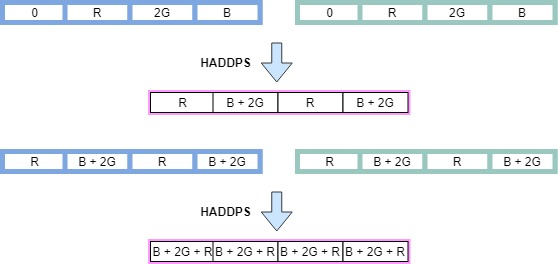
\includegraphics[scale=0.5]{img/haddps.jpg}
	\caption{Diagrama de operar con la instrucción HADDPS}
	\label{sumah}
  \end{center}
\end{figure}

{\centering\textbf{Procesado de los pixeles [i][j] y [i][j+1]:}}

Se cargan en un registro\textbf{XMM} 2 pixeles (8 bytes) de la imagen \textbf{src}.
Se desempaqueta la parte baja de byte a word, luego se guarda una copia del registro, y se desempaqueta cada componente de word a doubleword, sólo que para un registro la parte baja y para el otro la parte alta. \\
Obteniendo los valores de los componentes del pixel [i][j] en un registro y los de [i][j+1] en el otro. Y se convierten a float. \\
Luego se multiplica cada uno por los valores de \textbf{[mul09]}. 
Y se suma el registro que contiene 4 floats con el valor b/2 previamente calculado. \\
Luego se convierten los registros a datos enteros, se empaquetan a word y luego a byte sin signo y con saturación, obteniendo los valores esperados. \\
Finalmente se escriben en la imagen \textbf{dst}.
\begin{codesnippet}
\begin{verbatim}
        dst_matrix[i][j].r = SATURAR(src_matrix[i][j].r * 0.9 + b/2);
        dst_matrix[i][j].g = SATURAR(src_matrix[i][j].g * 0.9 + b/2);
        dst_matrix[i][j].b = SATURAR(src_matrix[i][j].b * 0.9 + b/2);
\end{verbatim}
\end{codesnippet}
\begin{figure}[ht]
  \begin{center}
	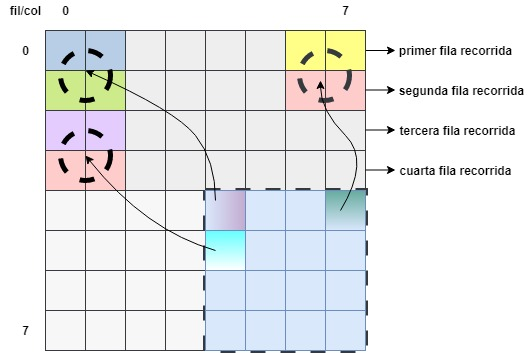
\includegraphics[scale=0.5]{img/fantasma1.jpg}
	\caption{Representación parcial de aplicar b/2 a cada pixel con el máximo valor de offset de X e Y}
	\label{calcb}
  \end{center}
\end{figure}

Llegando al final del ciclo, se avanzan los punteros dos pixeles de las imágenes \textbf{src} y \textbf{dst}, se evalúan los saltos condicionales para saber si ya no quedan pixeles por procesar, o si se continúa pero cambiando la fila de la matriz fantasma o si se vuelve al inicio de esta.

\newpage
\subsection{Color Bordes}
La finalidad de este filtro es la detección de bordes de la imagen sobre los pixeles lindantes de cada pixel, para eso calcula las diferencia tanto del eje horizontal como del vertical de los 8 pixeles y luego las suma. En este caso se deja un marco de 1 pixel de color blanco alrededor de toda la imagen, por lo que nos ahorramos los problemas de los casos borde.

\subsubsection{Pseudocódigo del ciclo:}
\begin{codesnippet}
\begin{verbatim}
Para i de 1 a height - 2;
    Para j de 1 a width - 2; 
        r=0, g=0, b=0;
        Para ii de i-1 a i+1
            r += abs(src_matrix[ii][j-1].r - src_matrix[ii][j+1].r);
            g += abs(src_matrix[ii][j-1].g - src_matrix[ii][j+1].g);
            b += abs(src_matrix[ii][j-1].b - src_matrix[ii][j+1].b);
        Para jj de j-1 a j+1
            r += abs(src_matrix[i-1][jj].r - src_matrix[i+1][jj].r);
            g += abs(src_matrix[i-1][jj].g - src_matrix[i+1][jj].g);
            b += abs(src_matrix[i-1][jj].b - src_matrix[i+1][jj].b);
        dst_matrix[i][j].r = SATURAR(r);
        dst_matrix[i][j].g = SATURAR(g);
        dst_matrix[i][j].b = SATURAR(b);
\end{verbatim}
\end{codesnippet}

\subsubsection{Implementación del ciclo en ASM}

Dado que alrededor de la imagen va a haber un marco de 1 pixel blanco, se declara una variable para dejar cuatro pixeles en blanco y otro para setear la transparencia en 255 para dos pixeles.
\begin{codesnippet}
\begin{verbatim}   
    blanco: TIMES 4 db 255, 255, 255, 255
    transparencia: TIMES 2 db 0, 0, 0, 255
\end{verbatim}
\end{codesnippet}

En cada ciclo se debe operar con los pixeles lindantes del pixel [i],[j], aprovechando el tamaño de los registros \textbf{XMM} se cargaran en 3 de estos 15 bytes, es decir4 pixeles, un registro para cada fila [i], [i-1] e [i+1] lo que permitirá procesar de a dos pixeles la imagen \textbf{dst}, porque para cada pixel se necesitan tanto los pixeles de la columna y fila anterior como los de las siguientes, al procesar de a dos pixeles se necesita 4 pixeles en lugar de 3 de cada fila. En la figura %~\ref{algo}\\
El registro con el que se hace el recorrido de la imagen \textbf{src} en el ciclo apunta al pixel [0][0], haciendo referencia a el pixel [i-1][j-1] en el pseudocódigo, que avanzará 2 pixeles en cada ciclo en mayor parte. En cambio cuando se esté a 4 pixeles del final de la fila, se avanzará 4 pixeles, comenzando el ciclo en una nueva fila. \\ Aprovechando el parámetro \textbf{src_row_size} se leen los pixeles de las filas inferior y superior correspondientes a las posiciones [i][j-1] y [i+1][j-1]. \\
El registro con el que se hace el recorrido de la imagen \textbf{dst}, luego de hacer el marco superior, apunta a la posición [1][1], y cada vez que se escriben los valores en el imagen, se avanza los dos pixeles siguientes hasta llega 3 pixeles antes del final de la fila, en ese caso se  avanza 4 pixeles, que se corresponde con la posición [i+1][1].
Cada vez que se está por cambiar de fila, se pone en blanco el último pixel de la fila, se pasa a la siguiente fila y se pone en blanco el primer pixel también. \\
El final del ciclo llega cuando no quedan más filas por recorrer.
En realidad queda una fila por recorrer pero esta se corresponde con el marco inferior, y se procede al igual que con el marco superior.
de los casos borde.  \\

{\centering\textbf{Preparación cálculo ii y jj:}}

Se realizará una copia de cada registro \textbf{XMM} que contiene los pixeles de las 3 filas consecutivas, para poder extender los componentes B,G,R,A de cada pixel a tamaño word. \\
Y se procederá a copiar los registros necesarios con estos nuevos componentes de tamaño word para el cálculo de jj y no tener que volver a leerlos de memoria. \\


{\centering\textbf{Cálculo ii:}}

Ahora con los componentes de tamaño word se procede a sacar las diferencias de cada fila respecto a las columnas [ii][j-1] y [ii][j+1] con las instrucciones \textbf{PSUBW} y \textbf{PABSW}. \\
Para luego hacer la sumatoria de estas diferencias con \textbf{PADDW}. \\

{\centering\textbf{Cálculo jj:}}

Se procede a sacar las diferencias de cada columna de las filas [i-1][jj] e [i+1][jj] con las instrucciones \textbf{PSUBW} y \textbf{PABSW}.
Ahora en este caso, en un registro \textbf{XMM} se tendrán las siguientes diferencias  abs([i-1][j-1]-[i+1][j-1]) y abs([i-1][j]-[i+1][j]), y en otro  abs([i-1][j+1]-[i+1][j+1]) y abs([i-1][j+2]-[i+1][j+2]), por lo que hay datos demás para los pixeles que se van a escribir, es por eso que se deben separar datos y no falten ni sobren valores. \\ Para eso se hace una copia y shifts para obtener los resultados deseados como se puede obeservar en la figura%~\ref{}. \\

Se prosigue con la suma de los valores finales de ii y jj, para luego unirlos mediante la instrucción \textbf{POR} con los valores de [\textbf{transparencia}]. Finalmente se cargan los datos en la imagen \textbf{dst} y se procede al siguiente ciclo o su salida.


\subsection{Reforzar Brillo}
\subsubsection{Pseudocódigo del ciclo:}
Este filtro aumenta y disminuye el brillo de la imagen mediante un cálculo respecto al brillo de cada pixel de la imagen \textbf{src}. \\
Para eso el filtro posee 4 parámetros de entrada del tipo entero: \textbf{umbralSup}, \textbf{umbralInf}, \textbf{brilloSup} y \textbf{brilloInf}. Si el cálculo queda fuera del rango de los umbrales su brillo aumenta o disminuye en caso de estar por encima del umbral superior o por debajo del inferior respectivamente, cabe aclarar que tanto el aumento y disminución se harán de forma saturada y por separado, para luego mediante una máscara se definirá si se aplican o no a los pixeles de la imagen \textbf{dst}. \\
En cambio si está dentro del rango de los umbrales su brillo no cambia.
\begin{codesnippet}
\begin{verbatim}
Para i de 0 a height - 1;
    Para j de 0 a width - 1; 
        b = (src_matrix[ii][jj].r + 2 * src_matrix[ii][jj].g + src_matrix[ii][jj].b) / 4;
        Si b > umbralSup:
            dst_matrix[i][j].b = SATURAR(src_matrix[i][j].b + brilloSup)
            dst_matrix[i][j].g = SATURAR(src_matrix[i][j].g + brilloSup)
            dst_matrix[i][j].r = SATURAR(src_matrix[i][j].r + brilloSup)
        Sino, si umbralInf > b:
            dst_matrix[i][j].b = SATURAR(src_matrix[i][j].b - brilloInf)
            dst_matrix[i][j].g = SATURAR(src_matrix[i][j].g - brilloInf)
            dst_matrix[i][j].r = SATURAR(src_matrix[i][j].r - brilloInf)
        Sino:
            dst_matrix[i][j].b = src_matrix[i][j].b
            dst_matrix[i][j].g = src_matrix[i][j].g
            dst_matrix[i][j].r = src_matrix[i][j].r
\end{verbatim}
\end{codesnippet}
En este filtro hay que hacer un cálculo muy similar al del filtro fantasma que será utilizado para comparar con los umbrales, pero con valores enteros, entonces el valor de b se va a extender a double word, pero no es necesario convertirlo a float.
La idea es que en cada ciclo se procesan las imágenes de a dos pixeles. \\

{\centering\textbf{Cálculo de b:}}

Se cargan los dos pixeles de la imagen \textbf{src} en un registro \textbf{XMM}, y se extiende a tamaño word. De esta forma los dos pixeles ocupan cada word del registro y no pierdo precisión. \\
Se multiplica el valor de los componente G con una máscara de words y deje en 0 el valor los words asociados a la transparencia y el resto no los modifique. \\
Luego se suman cada componente de forma horizontal con \textbf{PHADDW} 2 veces, teniendo un registro fuente repleto de 0's. \\
Finalmente se divide por 4 con otra máscara de words, obteniendo finalmente un registro \textbf{XMM} con los valores $|0|0|0|0|0|0|b|b|$. \\
Haciendo \textbf{PSHUFLW} extendemos b a double word, obteniendo  $|0|0|b|b|$ para poder comparar con los umbrales de tamaño double word. \\

{\centering\textbf{Preparación de los parámetros:}}

Como los umbrales \textbf{umbralSup} y \textbf{umbralInf} se deben comparar con el \textbf{XMM} = $|0|0|b|b|$, debe haber una correspondencia, por eso se cargan los umbrales de la forma $|0|0|umbral|umbral|$ en un registro para cada umbral \textbf{XMM}, esto se puede realizar haciendo moves y shift's o con un shuffle. \\

{\centering\textbf{Resta brilloInf:}}

Se carga de forma escalar el double word \textbf{brilloInf}, y se desempaqueta a word y luego a byte.
Lo siguiente es asignar a cada byte de la parte baja del registro \textbf{XMM}, el valor de \textbf{brilloInf} con la instrucción \textbf{PSHUFB}, excepto en los correspondientes a la componente de transparencia que tendrán ceros.
En una copia de los pixeles originales sin extender, se procede a restarles \textbf{brilloInf} a cada componente utilizando \textbf{PSUBUSB}. \\

{\centering\textbf{Suma brilloSup:}}

Se procede igual que con restaInf, obteniendo un registro \textbf{XMM} con cada byte de su parte baja el valor de \textbf{brilloSup} con la instrucción \textbf{PSHUFB}, dejando ceros en los byte correspondientes a la transparencia.
Y en una copia de los pixeles originales sin extender, se procede a sumarles \textbf{brilloSup} a cada componente utilizando \textbf{PADDUSB}. \\

{\centering\textbf{Comparación umbralInf $>$ b}}

Se utiliza \textbf{PCMPGTD} con el registro de \textbf{umbralInf} como destino y el b como fuente, el resultado será 0x00000000 en los double word que resulten menores o iguales a b y 0xffffffff para los mayores. \\

{\centering\textbf{Comparación b $>$ umbralSup:}}

Se compara usando \textbf{PCMPGTD} con el registro de b como destino y el de \textbf{umbralSup} como fuente, el resultado será 0x00000000 en los double word que resulten menores o iguales al umbral y 0xffffffff para los mayores.\\

{\centering\textbf{Selección de los valores correspondiente:}}

Con estos resultados, se hace un \textbf{PAND} a cada comparación con su correspondiente suma/resta de brillo, dejando en cero los componentes de los pixeles que no cumplían con su correspondiente condición. \\

{\centering\textbf{Caso b entre rango de umbrales}}

Para este caso, se unifican  los resultado de las comparaciones con un \textbf{POR}, y con la instrucción \textbf{PANDN} y los registros que tengan los valores de los pixeles originales se conservan aquellos en los que b se encuentra dentro del rango de ambos umbrales y quedan en 0 los que no.

\medskip

Finalmente se procede a hacer un \textbf{POR} de cada unos de los resultados de cada branch y con la máscara \textbf{[transparencia} se setea la componente A en 255.
Se repite el ciclo hasta que no queden más pixeles.

\subsection{Pixelado diferencial}
El efecto de pixelado diferencial divide la imagen en cuadrados de 4x4 pixeles, y determina si se deben copiar los 16 pixeles originales o el promedio de estos, según si la diferencia absoluta entre el cuadrado de 4x4 y el promedio supera un umbral dado por parámetro. \\

\medskip

El filtro se aplica a todos los pixeles, en este caso se procesa de a 16 pixeles, porque en caso de tener que pixelar les corresponden los mismos valores a cada pixel. 
Como se utilizan imágenes de un ancho múltiplo de 8, no hay problemas a la hora de recorrer cada fila. Pero puede o no haber problemas en las últimas filas de la imagen. Si la cantidad de filas no es múltiplo de 4, que se puede chequear con ayuda de los datos de entrada y agregar saltos para resolver ese caso particular dependiendo de las filas que queden por recorrer. \\
\subsubsection{Pseudocódigo del ciclo:}
\begin{codesnippet}
\begin{verbatim}
Para i de 0 a height - 1;
    Para j de 0 a width - 1; 
        -- Paso 1 Promedio pixeles
        r=0, g=0, b=0;
        Para ii de i a i+3
            Para jj de j a j+3
                r = r + src_matrix[ii][jj].r
                g = g + src_matrix[ii][jj].g
                b = b + src_matrix[ii][jj].b
        b = SATURAR(b/16)
        g = SATURAR(g/16)
        r = SATURAR(r/16)
        -- Paso 2 Calculo de diferencia
        value = 0
        Para ii de i a i+3
            Para jj de j a j+3
                value += abs(r - src_matrix[ii][jj].r) + abs(g - src_matrix[ii][jj].g) 
                + abs(b - src_matrix[ii][jj].b);
        Paso 3 Aplicacion segun umbral
        Si value < limit:
            Para ii de i a i+3
                Para jj de j a j+3
                    dst_matrix[ii][jj].b = src_matrix[ii][jj].b
                    dst_matrix[ii][jj].g = src_matrix[ii][jj].g
                    dst_matrix[ii][jj].r = src_matrix[ii][jj].r
        Sino:
            Para ii de i a i+3
                Para jj de j a j+3
                    dst_matrix[ii][jj].b = b
                    dst_matrix[ii][jj].g = g
                    dst_matrix[ii][jj].r = r
        j = j+4;
    i = i+4;
\end{verbatim}
\end{codesnippet}

\subsubsection{Idea general del ciclo en ASM}

En cada ciclo se cargarán en 4 registros \textbf{XMM} 16 bytes de la imagen correspondientes a 4 filas consecutivas, es decir 4 pixeles en cada registro. \\
Luego se desempaquetan a word tanto su parte alta como baja de los registros \textbf{XMM}, por lo que se tendrán 8 registros \textbf{XMM} con los valores de 2 pixeles cada uno.\\

{\centering\textbf{Cálculo del promedio:}}

Para el promedio simplemente se suman todos los registros con la instrucción \textbf{PADDW}, se suma la parte alta con la parte baja del registro y se divide por 16 la word usando \textbf{PSRLW} y el inmediato con el valor 4, que serán la cantidad de bits que cada word se shifteará a derecha.
Finalmente se copia la parte baja del registro con los promedios a su parte alta.

{\centering\textbf{Cálculo de la diferencia:}}

Se utilizará un registro \textbf{XMM} como acumulador, realizando una sumatoria de los resultados de varias operaciones.\\
Estas operaciones consistirán en calcular la diferencia del promedio con cada uno de los 16 pixeles, para ello habrá una copia de este y los pixeles para conservar su valor original, y luego se procederá a restarle uno de los pixeles extendidos a 8 bytes, se toma el valor absoluto y se suman las componentes entre sí para finalmente sumar el resultado al registro acumulador usando \textbf{PADDW}. \\
Esto para cada uno de los 16 pixeles, en realidad 8 de estos a la parte baja y los otros 8 a la parte alta del registro del promedio.  \\
Finalmente se suman la parte alta con la parte baja del promedio, terminando con la acumulación. \\

{\centering\textbf{Aplicación según umbral:}}

Se empaqueta el registro promedio de word a byte sin signo y con saturación. \\
Usando \textbf{MOVD} y \textbf{PSLLDQ} se ubicará cada valor de value (registro acumulador) en los 2 quad words del registro, lo mismo se hará con el dato de entrada entero \textbf{limit}. \\
De esta forma haciendo pcmpgtq se obtendrá un registro repleto de 1's o 0's, dependiendo si value es mayor a \textbf{limit} o menor en ese orden. \\
Luego hago un \textbf{PAND} entre los promedios y la máscara obtenida. 
Continuamos haciendo \textbf{PANDN} con la máscara y los pixeles originales en caso de que la condición no se cumpla. \\
Se combinan los resultados haciendo un \textbf{POR}, obteniendo los valores pixelados o lo originales según el resultado de las comparación.\\
Por último se escribe a memoria de a 4 pixeles por fila realizando \textbf{MOVDQU}, se repite el ciclo o se termina.


\section{Experimentación}
\subsection{Información relevante}:
En una computadora siempre hay varios procesos que están en ejecución, aunque no en simultáneo debido a la velocidad en la que trabajan los procesadores no es algo que podamos percibir dando esta sensación de continuidad, sino que mientras uno está siendo ejecutado los demás esperan para que sea su turno, ya sea porque el anterior proceso terminó o pasará a la lista de espera con los demás procesos.Al menos esto sucede en procesadores de un sólo core, los multi-core pueden correr más tareas en simultáneo, pero aún así siempre va a haber un gran número de tareas en espera, o puede llegar una interrupción que debe ser atendida.

Para analizar las implementaciones experimentales se tomaron medidas de tiempo (ciclos de reloj y microsegundos). 
Los ciclos de reloj se tomaron con con el soporte de la instrucción \textbf{rdtsc} que permite obtener el valor del \textbf{Time Stamp Counter} (TSC) del procesador. Que es un registro que aumenta con cada ciclo del procesador, la cátedra provee esta función, que retorna la diferencia entre la cantidad de ciclos antes y después del llamado al filtro, obteniendo la cantidad de ciclos de la ejecución.
Para tomar los microsegundos se utilizó la función \textbf{clock_gettime} que toma el tiempo en el momento específico en un buffer. De la misma forma en la que se calculan los ciclos de ejecución, se toman el tiempo inicial y final de la ejecución del ciclo y se calcula la diferencia en microsegundos.

Por el hecho de que hay varios procesos ejecutándose en cortos periodos de tiempo, no son exactas estas mediciones. Pero las mediciones se trataron de realizar lo más preciso posible y se tomó sólo la parte de ejecución del ciclo, no se tuvo en cuenta la carga y guardado de las imágenes Para cada experimento los filtros se ejecutaron 200 veces con imágenes de tamaño 1280x1024 pixeles. 
Los dos experimentos llevados a cabo son sobre la ImagenFantasma y con los offset máximos posibles.

También se corrieron bajo los comandos \textbf{nice} para que el programa tenga una mayor prioridad y \textbf{taskset} para asignarle un sólo core, de forma que sea menos probable que en un cambio de contexto sea desalojada, y se desaloje la asignada al otro core.

Los experimentos se corrieron con la ayuda de un script para que sea automatizado y no haya que hacer demasiadas manualidades junto con makefiles y \"copias\" modificadas del ejecutable tp2, para correr los filtros experimentales y generar los datos necesarios para su análisis. 

Todo se realizó en una notebook con un procesador \textbf{Intel Pentium B980} doble núcleo con una frecuencia base 2,40 GHz.

\subsection{Experimentación ImagenFantasma con enteros}
\subsubsection{Hipótesis}
Este experimento consiste en realizar todos los cálculos posibles usando instrucciones que del tipo entero para cada pixel.
¿Por qué hacer esto? Bueno, las operaciones en enteros son usualmente más sencillas para el microprocesador, aunque trabajar de varios datos a la vez de seguro tiene un costo que de a un sólo dato, pero en cuanto al números de operaciones que se deberán realizar tiene mayor rendimiento.
A la hora de hacer cuentas, debido a los límites de una computadora en términos de precisión y tamaño de los datos que almacena, la hipótesis que es menos costoso y más rápido procesar números enteros que datos de punto flotante.
Además la idea surge porque los componentes de los pixeles son valores enteros (de 8 bits cada uno) y entonces de seguro no es necesario hacer todas sus operaciones en float, como el cálculo de b:
\begin{codesnippet}
\begin{verbatim}
        float b = (src_matrix[ii][jj].r + 2 * src_matrix[ii][jj].g + src_matrix[ii][jj].b) / 4;
\end{verbatim}
\end{codesnippet}
Esas operaciones se pueden hacer con operaciones de enteros, quizás se pierda algún dato al momento de la división. Quizás valga la pena en cuanto al rendimiento.
Entonces ¿Hay diferencias entre operar con enteros o punto flotantes? ¿Hay diferencias significativas en la imagen final? ¿Qué implementación es mejor?


\subsubsection{Resultados}
Con los datos obtenido de los tiempo de ejecución se realizaron los siguientes gráficos:

\begin{figure}[hb]
    \begin{center}
	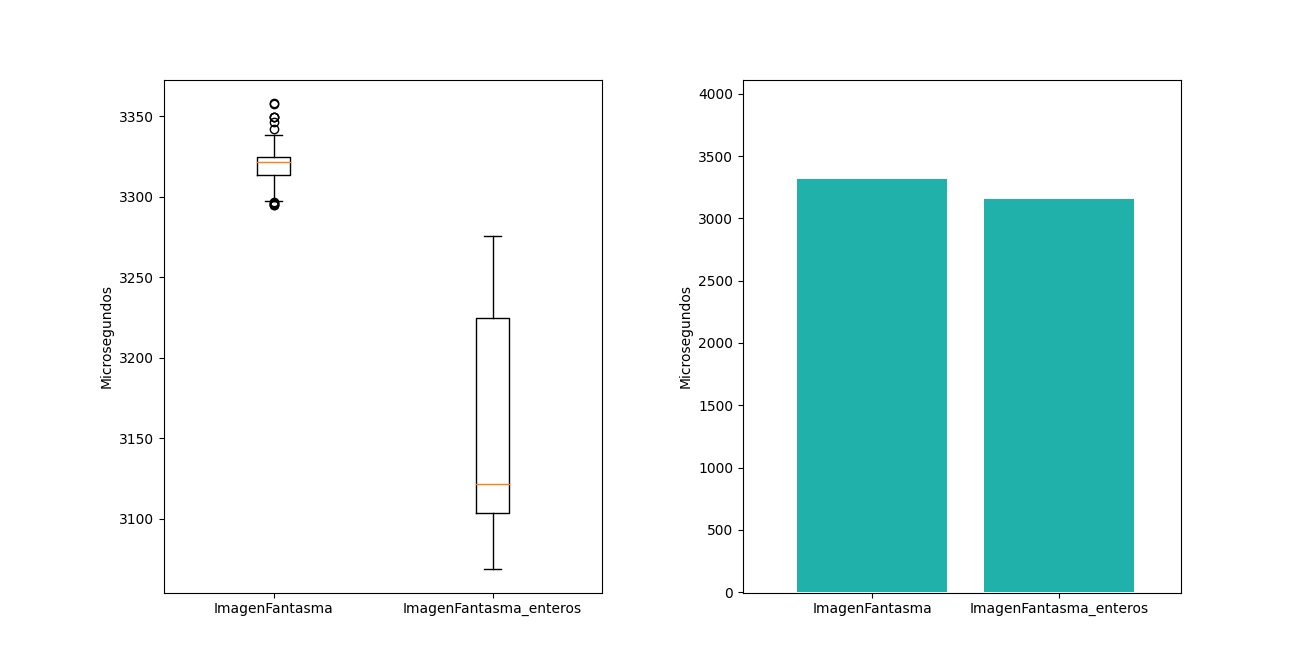
\includegraphics[scale=0.50]{img/enteros1.jpeg}
	\end{center}
	\caption{Dispersión y media microsegundos por ejecución}
	\label{exp1_m}
\end{figure}

Viendo el gráfico izquierdo, podríamos decir que no se ve una gran diferencia, ya que no tenemos una percepción justa en tiempo tan pequeños, pero viendo el gráfico de la derecha se puede decir que son bastante similares, la diferencia más o menos de 200 microsegundos es despreciable.

\begin{figure}
    \begin{center}
	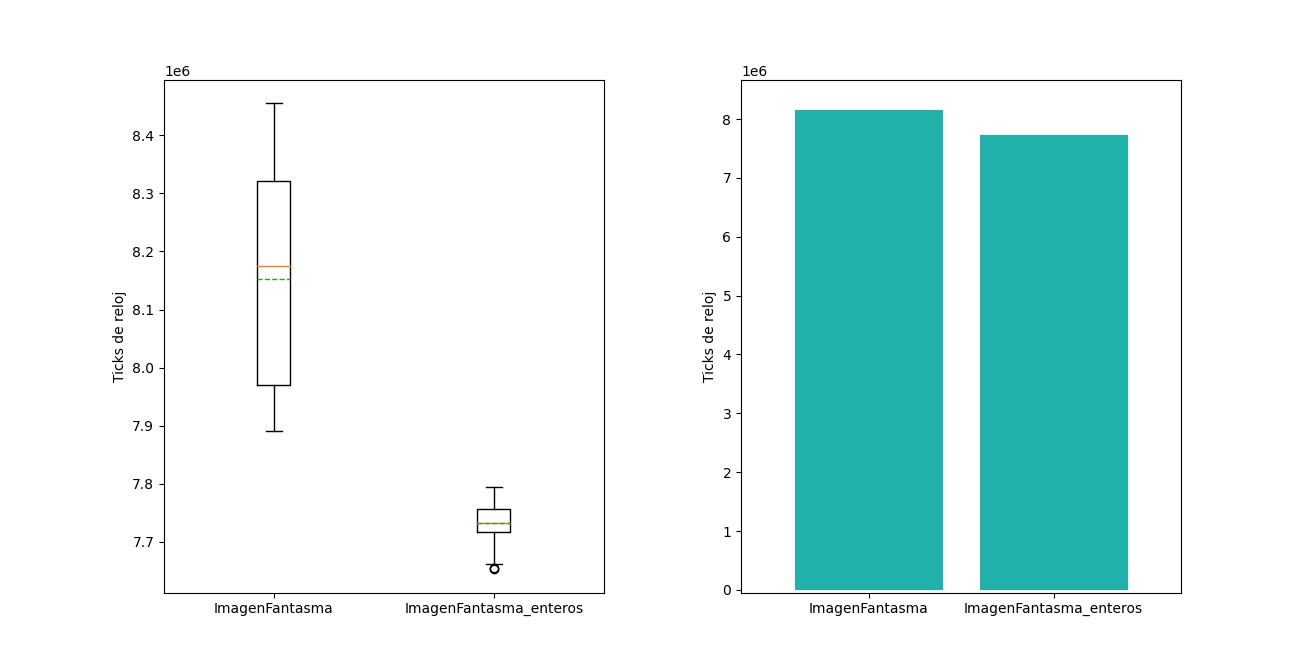
\includegraphics[scale=0.50]{img/enteros2.jpeg}
    \end{center}
	\caption{Dispersión y media de los ticks de reloj}
	\label{exp1_c}
\end{figure}

Pero con el gráfico de los ticks reloj se puede apreciar un poco más las diferencias dado que son más cuantificables. Los boxplot muestran que las operaciones con float llevan a que los tiempos tengan una media de poco más 8 millones en mayor parte. En cuanto a las operaciones en enteros los valores rondan por debajo de los 8 millones, con una media de alrededor de los 7.75 millones de ticks de reloj.

\subsubsection{Conclusión}
Dado los resultados se concluye que la hipótesis es correcta, como se esperaba. Aunque no se ve una diferencia muy grande, ambas implementaciones tienen un comportamiento similar.
Probablemente se deba al siguiente extracto del pseudocódigo:
\begin{codesnippet}
\begin{verbatim}
    dst_matrix[i][j].r = SATURAR(src_matrix[i][j].r * 0.9 + b/2);
    dst_matrix[i][j].g = SATURAR(src_matrix[i][j].g * 0.9 + b/2);
    dst_matrix[i][j].b = SATURAR(src_matrix[i][j].b * 0.9 + b/2);
\end{verbatim}
\end{codesnippet}
El multiplicar por 0.9, que es un número flotante, es una operatoria que no podemos realizar con números enteros y tampoco existe una instrucción que divida con enteros en \textbf{SIMD}, es por eso que a pesar del cálculo de b se haya realizado con operaciones en enteros aún se tuvo que extender cada componente de los pixeles a tamaños de 4 bytes para luego convertirlos en floats y luego volver a convertirlos en enteros, y reducirlos a tamaño byte, en toda ese proceso es donde creo que se encuentra el límite de la mejora de performance para esta implementación.


\subsection{Experimentación ImagenFantasma de a 4 pixeles}
\subsubsection{Hipótesis}
¿Operar con más datos mejora el rendimiento de un programa? Depende, si realiza la misma cantidad de instrucciones no se esperaría que cambie.
En nuestro caso, ¿Y si la cantidad de instrucciones ejecutadas por pixel en cada ciclo es menor? ¿O hay más instrucciones por ciclo, pero hay menos accesos a memoria?
El planteamiento de este experimento es tratar de responder ambas preguntas.

Como expliqué en el desarrollo del filtro ImagenFantasma y como muestra la figura~\ref{calcb}, si dividimos la imagen a procesar en submatrices de 2x2, el cálculo de b tiene datos en común para toda la submatriz, estos son los pixeles presentes en la submatriz correspondiente a los offset.
Entonces en lugar de procesar de a dos pixeles, y recorrer cada fila de la submatriz de los offsets dos veces  por ciclo, es decir dos veces cada pixel.
Esta implementación recorre la imagen como una matriz de submatrices de 2x2 y ya no recorre las filas de la submatriz más de una vez.
Planteado el caso, se espera que la perfomance del filtro mejore.

\subsubsection{Resultados}
\begin{figure}[h]
    \begin{center}
	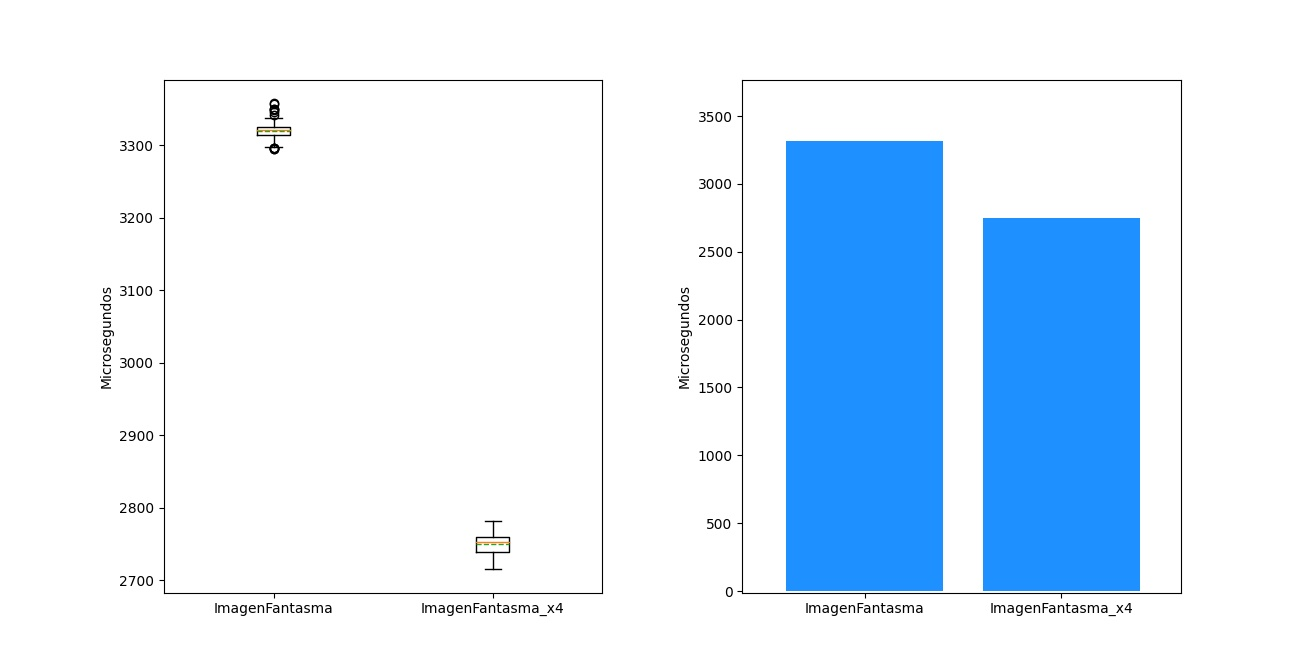
\includegraphics[scale=0.55]{img/x41.jpeg}
	\end{center}
	\caption{Dispersión y media de ejecución en microsegundos}
	\label{exp2_m}
\end{figure}
Viendo cómo se distribuyen los microsegundos para el filtro normal y el experimental, se puede apreciar una mejoría de alrededor unos 600 microsegundos teniendo en referencia los 3300 que toma el filtro original. De nuevo es difícil de apreciar por la medida de tiempo pero es significativa.

\begin{figure}[!h]
    \begin{center}
	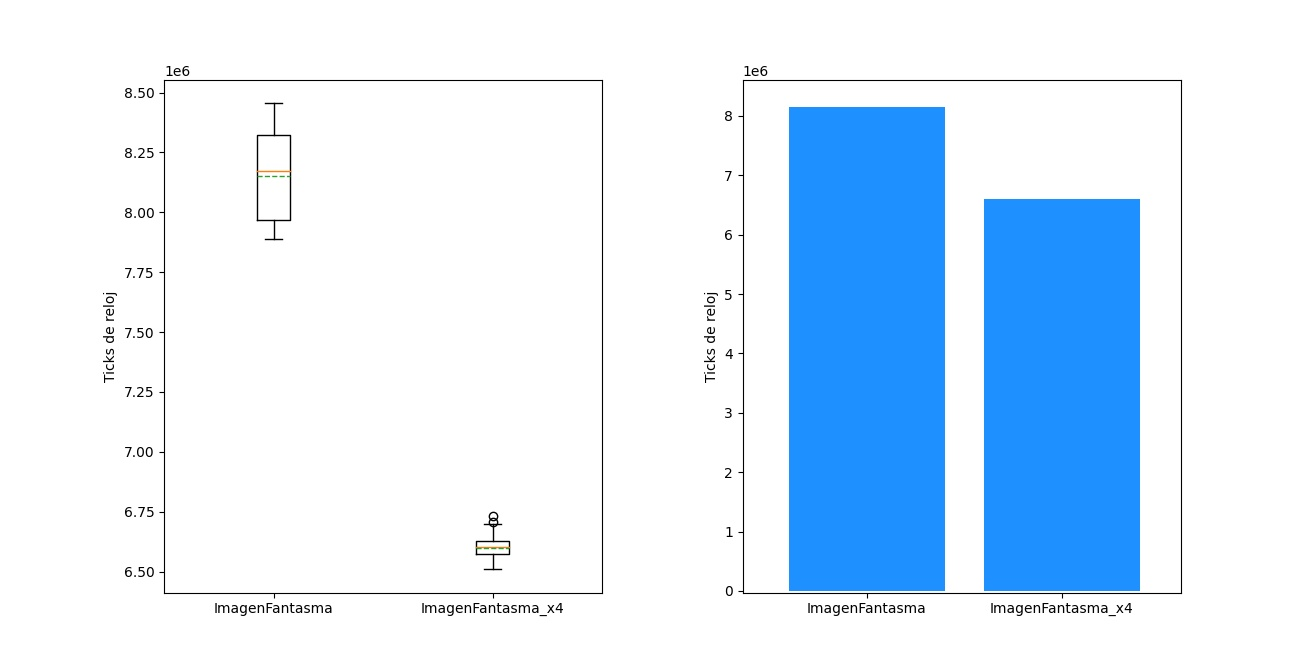
\includegraphics[scale=0.55]{img/x42.jpeg}
	\end{center}
	\caption{Dispersión y media de los ticks reloj por ejecución}
	\label{exp2_c}
\end{figure}

En cuanto a los ticks de relojs, el filtro que procesa de a 4 pixeles ronda en los 6 millones y medio de clocks, a diferencia de los 8.25 millones que toma el filtro normal.
La mejora de performance es notable.

\subsubsection{Conclusión}
 Los resultados son los esperados. La cantidad de instrucciones por ciclo es mayor, pero al realizar los cálculos relacionados a la submatriz de offsets, se reducen los accesos a memoria a la mitad, junto a los ciclos de procesar la imagen completa. Y los datos en los gráficos son la prueba de eso.
    

\section{Conclusión}
Llegando al final del trabajo, podemos concluir que el modelo de procesamiento vectorial es una gran herramienta para trabajar con muchos datos que deben ser procesados por igual. Por lo general nos permite reducir la cantidad de iteraciones que los que haríamos con operaciones \textbf{SISD}, y permitiéndonos tener una mejor precisión para los datos de punto flotante. 
Aunque tiene cierta dificultad, al no estar habituado al modelo, como saber interpretar cuál es el estado de los registros que uno usa, que contienen, que representan y cómo manipularlos, puede ser muy fácil equivocarse y obtener resultados no deseados. Lo mismo con los accesos a memoria, hay que tener la certeza de acceder a datos que nos sean accesibles.
Teniendo todo eso presente, el modelo de programación vectorial es sumamente efectivo para aplicaciones multimedia.
\end{document}

